\documentclass[tikz,border=2pt]{standalone}
\usepackage{amsmath}
\usetikzlibrary{arrows.meta}
\begin{document}
% Two-level bonus-malus system: premium c after a claim-free year, 2c after a year with claims;
% next level depends only on whether the annual count N_t is zero (probability e^{-lambda}).
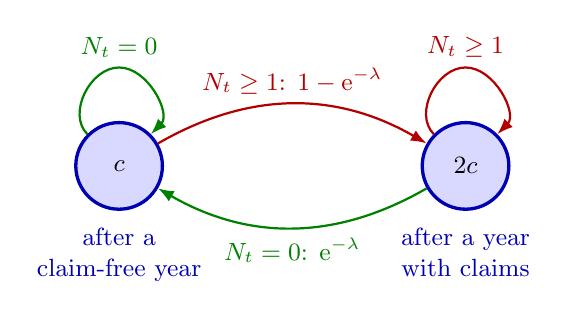
\begin{tikzpicture}[font=\small, >={Latex[length=2mm]},
  lev/.style={circle, draw=blue!70!black, very thick, fill=blue!15, minimum size=11mm}]
  \node[lev] (lo) at (0,0) {$c$};
  \node[lev] (hi) at (4.4,0) {$2c$};
  \node[blue!70!black, below=1mm, align=center] at (lo.south) {after a\\claim-free year};
  \node[blue!70!black, below=1mm, align=center] at (hi.south) {after a year\\with claims};
  % transitions
  \draw[->, thick, red!70!black] (lo) to[bend left=30] node[above, align=center] {$N_t\ge1$: $1-\mathrm{e}^{-\lambda}$} (hi);
  \draw[->, thick, green!50!black] (hi) to[bend left=30] node[below] {$N_t=0$: $\mathrm{e}^{-\lambda}$} (lo);
  \draw[->, thick, green!50!black] (lo.north west) to[out=135, in=180, looseness=1.0] (0,1.25) to[out=0, in=45, looseness=1.0] (lo.north east);
  \node[green!50!black, anchor=south] at (0,1.25) {$N_t=0$};
  \draw[->, thick, red!70!black] (hi.north west) to[out=135, in=180, looseness=1.0] (4.4,1.25) to[out=0, in=45, looseness=1.0] (hi.north east);
  \node[red!70!black, anchor=south] at (4.4,1.25) {$N_t\ge1$};
\end{tikzpicture}
\end{document}
